\documentclass[a4paper, 12pt]{extarticle}

% Поля
%--------------------------------------
\usepackage{geometry}
\geometry{a4paper,tmargin=2cm,bmargin=2cm,lmargin=3cm,rmargin=1cm}
%--------------------------------------


%Russian-specific packages
%--------------------------------------
\usepackage[T2A]{fontenc}
\usepackage[utf8]{inputenc} 
\usepackage[english, main=russian]{babel}
%--------------------------------------

\usepackage{textcomp}

% Красная строка
%--------------------------------------
\usepackage{indentfirst}               
%--------------------------------------             


%Graphics
%--------------------------------------
\usepackage{graphicx}
\graphicspath{ {./images/} }
\usepackage{wrapfig}
\usepackage{minted}
%--------------------------------------

% Полуторный интервал
%--------------------------------------
\linespread{1.3}                    
%--------------------------------------

%Выравнивание и переносы
%--------------------------------------
% Избавляемся от переполнений
\sloppy
% Запрещаем разрыв страницы после первой строки абзаца
\clubpenalty=10000
% Запрещаем разрыв страницы после последней строки абзаца
\widowpenalty=10000
%--------------------------------------

%Списки
\usepackage{enumitem}

%Подписи
\usepackage{caption} 

%Гиперссылки
\usepackage{hyperref}

\hypersetup {
	unicode=true
}

%Рисунки
%--------------------------------------
\DeclareCaptionLabelSeparator*{emdash}{~--- }
\captionsetup[figure]{labelsep=emdash,font=onehalfspacing,position=bottom}
%--------------------------------------

\usepackage{tempora}
\usepackage{amsmath}
\usepackage{color}
\usepackage{listings}
\lstset{
  belowcaptionskip=1\baselineskip,
  breaklines=true,
  frame=L,
  xleftmargin=\parindent,
  language=Python,
  showstringspaces=false,
  basicstyle=\footnotesize\ttfamily,
  keywordstyle=\bfseries\color{blue},
  commentstyle=\itshape\color{purple},
  identifierstyle=\color{black},
  stringstyle=\color{red},
}

%--------------------------------------
%			НАЧАЛО ДОКУМЕНТА
%--------------------------------------

\begin{document}

%--------------------------------------
%			ТИТУЛЬНЫЙ ЛИСТ
%--------------------------------------
\begin{titlepage}
\thispagestyle{empty}
\newpage


%Шапка титульного листа
%--------------------------------------
\vspace*{-30 pt}
\hspace{-65pt}
\begin{minipage}{0.3\textwidth}
\hspace*{-20pt}\centering

\includegraphics[width=60pt]{emblem}
\end{minipage}
\begin{minipage}{0.67\textwidth}\small \textbf{
\vspace*{-0.7ex}
\hspace*{-6pt}\centerline{Министерство науки и высшего образования Российской Федерации}
\vspace*{-0.7ex}
\centerline{Федеральное государственное бюджетное образовательное учреждение }
\vspace*{-0.7ex}
\centerline{высшего образования}
\vspace*{-0.7ex}
\centerline{<<Московский государственный технический университет}
\vspace*{-0.7ex}
\centerline{имени Н.Э. Баумана}
\vspace*{-0.7ex}
\centerline{(национальный исследовательский университет)>>}
\vspace*{-0.7ex}
\centerline{(МГТУ им. Н.Э. Баумана)}}
\end{minipage}
%--------------------------------------

\vspace{10pt}
\hspace{-35pt} \noindent \small ФАКУЛЬТЕТ\hspace{80pt} <<Информатика и системы управления>>

\vspace*{-16pt}
\hspace{47pt}\rule{0.83\textwidth}{0.4pt}

\vspace{0.5ex}
\hspace{-35pt} \noindent \small КАФЕДРА\hspace{50pt} <<Теоретическая информатика и компьютерные технологии>>

\vspace*{-16pt}
\hspace{30pt}\rule{0.866\textwidth}{0.4pt}
  
\vspace{6em}

\begin{center}
\Large {\bf Лабораторная работа №8} \\ 
\large {\bf по курсу <<Языки и методы программирования>>} \\ 
\large «Разработка шаблона класса» \\
\large <<Вариант 16>>
\end{center}\normalsize

\vspace{15em}


\begin{flushright}
  {Студент группы ИУ9-21Б: Пенкин А. Д.\hspace*{15pt} \\
  \vspace{2ex}
  Преподаватель: Посевин Д. П.\hspace*{15pt}}
\end{flushright}

\bigskip

\vfill
 \vspace{7em}

\begin{center}
\textsl{Москва 2023}
\end{center}
\end{titlepage}
%--------------------------------------
%		КОНЕЦ ТИТУЛЬНОГО ЛИСТА
%--------------------------------------

\renewcommand{\ttdefault}{pcr}

\setlength{\tabcolsep}{3pt}
\newpage
\setcounter{page}{2}

\section{Цель}\label{Sect::task}
\par
Целью данной работы является изучение шаблонов классов языка C++. 
\section{Условие}
\par
Matrix<T,N> – квадратная матрица размера N, элементы которой имеют тип T. Матрица должна иметь следующие операции:
1. запись значения в элемент с индексами (i, j);
2. чтение значения из элемента с индексами (i, j);
3. построение новой матрицы путём удаления iтой строки и j-того столбца. В Matrix<bool,N> при N ≤ 8 матрица должна быть представлена 64-разрядным целым числом, в котором каждому элементу соответствует один бит. 
\par
Последовательность символов ASCII с операциями:
1. получение количества символов;
2. получение ссылки на i-тый символ;
3. вставка нового символа в i-тую позицию
последовательности;
4. проверка, является ли последовательность
палиндромом. 
\section{Код решения}
1. lab8.cpp
\begin{minted}{c++}
#include <iostream>
#include "Matrix.h"
#include <math.h>
#include <string>
#include <vector>


int main()
{
	std::cout << "define new int matrix with dim 10:\n";
	Matrix<int, 10>* a = new Matrix<int, 10>(0);
	a->printMatrix();

	std::cout << "\n\n set some values in matrix: \n";

	a->setValue(1, 3, 12);
	a->setValue(2, 4, 1);
	a->setValue(4, 0, 3);
	a->setValue(8, 5, -4);
	a->setValue(5, 9, 55);

	a->printMatrix();

	std::cout << "\n\n element from position(1, 3): " << a->getValue(1, 3);

	Matrix<int, 9>* b = a->minor(1, 1);

	std::cout << "\n\n minor from (1, 1):\n";
	b->printMatrix();

	std::cout << "\n\n string matrix:\n";
	Matrix<std::string, 8>* c = new Matrix<std::string, 8>("WOW");
	c->printMatrix();
}
\end{minted}
2. Matrix.h
\begin{minted}{c++}
#pragma once
#include <iostream>
#include <vector>
#include <math.h>
#include <string>

template <typename T, int N>
class Matrix
{
private:
	std::vector<std::vector<T>> a;
	long long a1;
public:
	Matrix(T x);
	bool isBoolSmall;
	void print();
	void printMatrix();
	void setValue(int a, int b, T v);
	T getValue(int a, int b);
	Matrix<T, N - 1>* minor(int a, int b);
};

template <typename T, int N>
void Matrix<T, N>::print()
{
	std::cout << N << "\n";
}


template <typename T, int N>
Matrix<T, N>::Matrix(T x) {
	this->isBoolSmall = false;
	this->a1 = 0;
	this->a.resize(N);
	for (int i = 0; i < N; i++) {
		this->a[i].resize(N);
		for (int j = 0; j < N; j++) {
			this->a[i][j] = x;
		}
	}
}


template <typename T, int N>
void Matrix<T, N>::printMatrix() {
	if (this->isBoolSmall) {
		for (int i = 0; i < N; i++) {
			for (int j = 0; j < N; j++) {
				std::cout << (long long)(a1 / pow(2, (8 * i + j))) % 2 << " ";
			}
			std::cout << "\n";
		}
	}
	else {
		for (int i = 0; i < N; i++) {
			for (int j = 0; j < N; j++) {
				std::cout << a[i][j] << " ";
			}
			std::cout << "\n";
		}
	}
}


template <typename T, int N>
void Matrix<T, N>::setValue(int a, int b, T v) {
	if (this->isBoolSmall) {
		a1 |= (long long)pow(2, 8 * a + b);
		if (!v) {
			a1 /= (long long)pow(2, 8 * a + b);
		}
	}
	else {
		this->a[a][b] = v;
	}
}


template <typename T, int N>
T Matrix<T, N>::getValue(int a, int b) {
	if (this->isBoolSmall) {
		return (long long)(a1 / pow(2, (8 * a + b))) % 2 == 1;
	}
	else {
		return this->a[a][b];
	}
}


template <typename T, int N>
Matrix<T, N - 1>* Matrix<T, N>::minor(int x, int y) {
	Matrix<T, N - 1>* b = new Matrix<T, N - 1>(this->a[0][0]);
	if (b->isBoolSmall) {
		int m = 0, l = 0;
		for (int i = 0; i < N; i++) {
			if (i == x) { continue; }
			else { m++; }
			for (int j = 0; j < N; j++) {
				a1 *= (long long)pow(2, 8 * m + l);
			}
			std::cout << "\n";
		}
	}
	else {
		int m = 0, l = 0;
		for (int i = 0; i < N; i++) {
			if (i == x) { continue; }
			for (int j = 0; j < N; j++) {
				if (j == y) { continue; }
				b->setValue(m, l, a[i][j]);
				l++;
			}
			m++;
			l = 0;
		}
	}
	return b;
}
\end{minted}

\section{Результаты работы программы}
\begin{figure}[H]
    \centering
    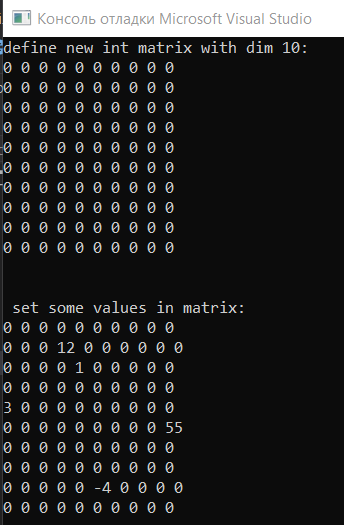
\includegraphics[width=400pt]{Test.png}
    \caption{создание и изменение матрицы}
    \label{fig:my_label}
\end{figure}

\begin{figure}[H]
    \centering
    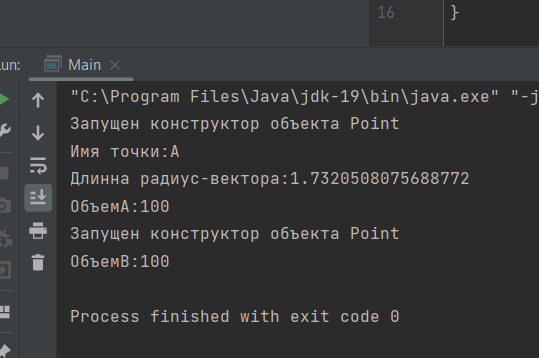
\includegraphics[width=400pt]{Test1.png}
    \caption{взятие элемента и минора}
    \label{fig:my_label}
\end{figure}

\begin{figure}[H]
    \centering
    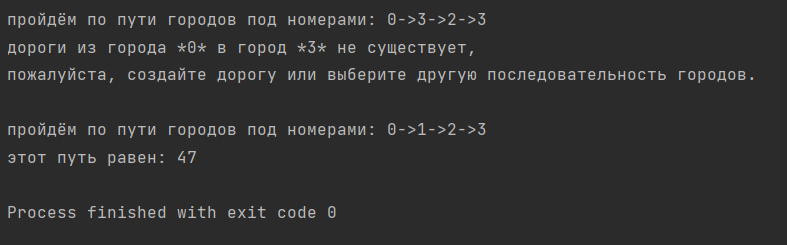
\includegraphics[width=400pt]{Test2.png}
    \caption{матрица строк}
    \label{fig:my_label}
\end{figure}


\end{document}